\chapter{Bonus: A Search for Milli-Charged Particles at the LHC}

\section{Motivation of a search for milli-charged particles}

One of the central mysteries of modern particle physics is the question of what
makes up dark matter. It must consist of massive particles that interact
at most very weakly with the SM, and no viable candidate exists among the
currently known particles. Moreover, a decade's worth of data from the LHC
has provided no evidence of any new particles that might provide an explanation.

We thus ask the question, what types of signatures might hypothetical dark matter
particles produce that would escape detection at present experiments?
One method of explaining dark matter is to add a new ``dark sector'' of
particles beyond the SM that couples only weakly to the SM. As an example,
we can add a ``dark photon'' $A'_\mu$ and a ``dark fermion'' $\psi'$ charged
under the new gauge field with charge $e'$. Allowing for kinetic
mixing between $A'_\mu$ and the SM weak hypercharge field $B_\mu$, the Lagrangian
for this new dark sector can be written
\be
\begin{split}
\mathcal{L}_\text{dark-sector} = &-\frac{1}{4}A'_{\mu\nu}A'^{\mu\nu} \\
&+i\bar{\psi}'(\gamma^\mu\partial_\mu + ie'\gamma^\mu A'_\mu + iM_\text{mCP})\psi' \\
&-\frac{\kappa}{2}A'_{\mu\nu}B^{\mu\nu},
\end{split}
\ee
where the first line is the kinetic term for a massless dark photon,
the second line contains the kinetic terms for a dark fermion with
mass $M_\mrm{mCP}$ as well as the interaction term with $A'_\mu$, and
the third line contains the mixing term between $A'_\mu$ and $B_\mu$, with
mixing strength parameter $\kappa$.

The mixing term can be eliminated by redefining $A'_{\mu\nu}\to A'_{\mu\nu}+\kappa B_{\mu\nu}$,
resulting in an interaction term $\kappa e'\bar{\psi}'\gamma^\mu B_\mu\psi$ between $\psi'$
and $B_\mu$. Rewriting $B_\mu$ in terms of the physical photon and $Z$ boson fields
as $B_\mu=\cos\theta_w A_\mu - \sin\theta_w Z_\mu$, we find that the new dark fermion
couples to the SM photon with electric charge $\kappa e'\cos\theta_w$, and couples to the 
SM $Z$ with charge $\kappa e'\sin\theta_w$. The mixing strength $\kappa$ must be small
(or else the new dark sector would have been observed already). so we must have
$\varepsilon\equiv \kappa e'\cos\theta_w \ll 1$, and we call $\psi'$ a
``milli-charged particle'' (mCP; note that the name is a bit of a misnomer because $\varepsilon$
does not have to be exactly O($10^{-3}$))

Such milli-charged particles have been searched for via a variety of methods,
either directly through collider experiments or indirectly through
solar effects, astronomical observations, or cosmological bounds.
A summary of the present exclusion space in the mCP mass--charge plane
is shown in Fig.~\ref{fig:mcp_search_status}, taken from~\cite{Vinyoles:mcp}.

\begin{figure}[t]
  \begin{center}
    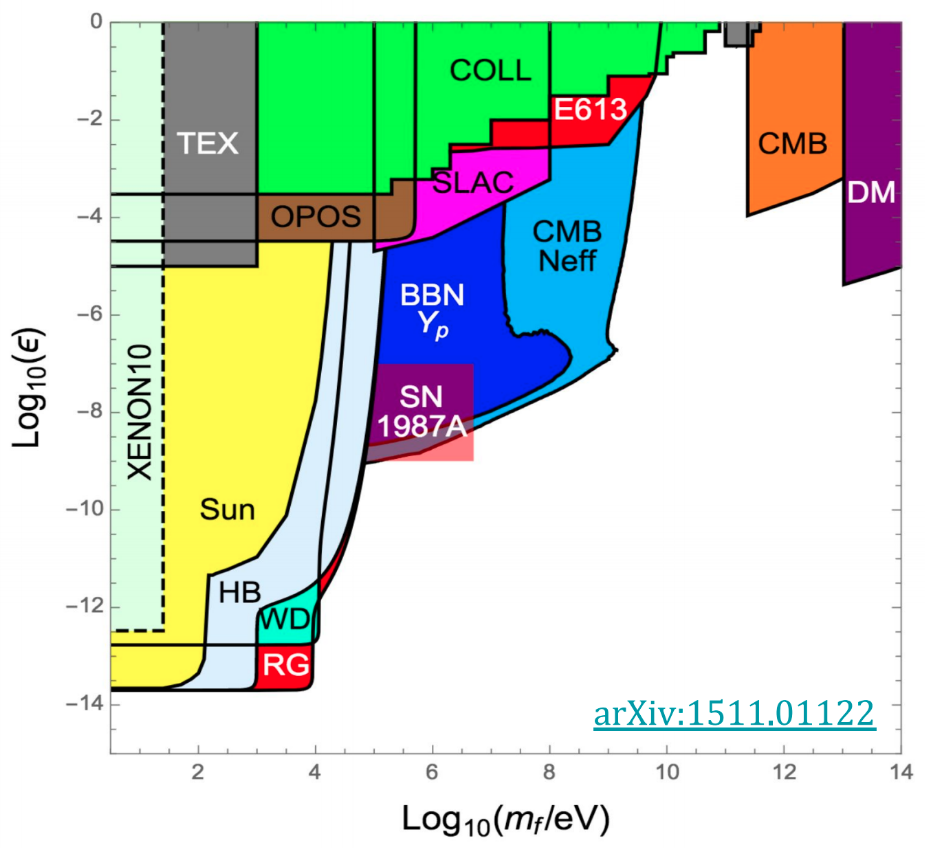
\includegraphics[width=0.50\textwidth]{figs/milliq/search_status.png}
    \caption{Existing exclusion limits for milli-charged partcles, coming
      from searches via colliders, solar effects, astronomical observations,
      and cosmological bounds. milliQan targets the unexcluded phase space
      with $\varepsilon\geq10^{-3}$ and $10^{-1} < m_\text{mCP} < 10^2\GeV$.
      (Image from~\cite{Vinyoles:mcp})
            }
    \label{fig:mcp_search_status}
  \end{center}
\end{figure}

There is a gap in the excluded phase space for $\varepsilon>10^{-3}$ at
the mass scales relevant at the LHC, roughly $10^{-1} < m_\text{mCP} < 10^2\GeV$.
mCPs at such masses and charges would be produced frequently at the LHC, but
present experiments would not be able to detect them; direct sensitvity is lost
for $\varepsilon$ below a few times $10^{-1}$, and a low cross sections
preclude missing energy searches. Therefore, a dedicated experiment is necessary
to search for mCPs at the LHC.


\section{Overview of the milliQan experiment}
The milliQan experiment, designed to search for mCPs using collisions at LHC P5, was proposed in 
2016~\cite{mq:loi}. It is located in a drainage gallery, elevated 45$^\circ$ above and 33
m from the CMS experiment. The proposed design consists of three stacked layers of plastic 
scintillator arrays, with each scintillating bar coupled to a photomultiplier tube (PMT).
The bars are sensitive enough to detect individual photoelectrons produced by
throughgoing mCPs, and requiring a hit in all three layers simultaneously drastically
reduces background, which mostly consists of random overlap of pulses from
PMT dark rate, environmental radiation, cosmic rays, and afterpulsing.


\section{Bench tests for PMT calibration}

\section{Generation of signal Monte Carlo}

